\documentclass{article}
\usepackage[spanish]{babel}
\usepackage{fancyhdr}
\usepackage{graphicx}
\usepackage{setspace}
\usepackage[table]{xcolor}
\usepackage{tabularx}
\usepackage{array}
\usepackage{multicol}
\usepackage{multirow}
\usepackage[margin=2.5cm]{geometry}
\usepackage{float}
\usepackage{color, colortbl}
\definecolor{tablebackground}{rgb}{0.8, 0, 0}


\newcolumntype{M}[1]{>{\centering\arraybackslash}m{#1}}
\newcolumntype{N}{>{\centering\arraybackslash}p{3.5cm}}
\newcolumntype{x}[1]{>{\centering\arraybackslash}p{#1}}

\pagestyle{fancy}
\lhead{\begin{picture}(0,0) \put(0,0){
\includegraphics[width=30mm]{img/logoSistemas.png}} \end{picture}}
\rhead{\begin{picture}(0,0) \put(-33,5){
\includegraphics[width=12mm]{./img/logoAbet.png}} \end{picture}}
\renewcommand{\headrulewidth}{0.5pt}

\fancyhead[C]{
 	\tiny Universidad Nacional de San Agustín de Arequipa \\
  	Facultad de Ingeniería de Producción y Servicios \\
  	Departamento de Ingeniería de Sistemas e Informática \\
  	Escuela Profesional de Ingeniería de Sistemas \\
  	\textbf{Programación Web 2}
}

\fancyfoot[L]{Estudiante Rafael Nina Calizaya}
\fancyfoot[C]{Pag. \thepage}
\fancyfoot[R]{Programación Web 2}
\renewcommand{\footrulewidth}{0.5pt}


\newcommand{\itemNombre}{Rafael Diego Nina Calizaya}
\newcommand{\itemCorreo}{rninacal@unsa.edu.pe}
\newcommand{\itemEscuela}{Escuela Profesional de Ingeniería de Sistemas}
\newcommand{\itemCurso}{Programación Web 2}
\newcommand{\itemSemestre}{III}
\newcommand{\itemCodigo}{1702122}
\newcommand{\itemLaboratorio}{04}
\newcommand{\itemTema}{NodeJS + Express}
\newcommand{\itemSemestreAcademico}{2024-A}
\newcommand{\itemInicio}{20 Mayo 2024}
\newcommand{\itemFinal}{24 Mayo 2024}

\begin{document}
.

\begin{center}	
	\fontsize{17}{17} \textbf{ Informe de Laboratorio \itemLaboratorio}
\end{center}
\centerline{\textbf{\Large Tema: NodeJS + Express}}

\begin{flushright}
	\begin{tabular}{|M{2.5cm}|N|}
		\hline
		\rowcolor{tablebackground}
		\color{white} \textbf{Nota}  \\
		\hline 
		     \\[18pt]
		\hline 			
	\end{tabular}
\end{flushright}	
\begin{table}[h]
	\renewcommand{\arraystretch}{0.5}
	\hspace{2px}
	\begin{tabular}{|x{4.8cm}|x{4.8cm}|x{4.8cm}|}
		\hline 
		\rowcolor{tablebackground}
		\color{white} \textbf{Estudiante} & \color{white}\textbf{Escuela}  & \color{white}\textbf{Asignatura}   \\
		\hline 
		{\itemNombre \par \itemCorreo} & \itemEscuela & {\itemCurso \par Semestre: \itemSemestre \par Código: \itemCodigo}     \\
		\hline 			
	\end{tabular}
\end{table}		
	
\begin{table}[h]
	\renewcommand{\arraystretch}{0.5}
	\hspace{2px}
	\begin{tabular}{|x{4.8cm}|x{4.8cm}|x{4.8cm}|}
		\hline 
		\rowcolor{tablebackground}
		\color{white}\textbf{Laboratorio} & \color{white}\textbf{Tema}  & \color{white}\textbf{Duración}   \\
		\hline 
		\itemLaboratorio & \itemTema & 06  \\
		\hline 
	\end{tabular}
\end{table}

\begin{table}[h]
	\renewcommand{\arraystretch}{0.5}
	\hspace{2px}
	\begin{tabular}{|x{4.8cm}|x{4.8cm}|x{4.8cm}|}
		\hline 
		\rowcolor{tablebackground}
		\color{white}\textbf{Semestre académico} & \color{white}\textbf{Fecha de inicio}  & \color{white}\textbf{Fecha de entrega}   \\
		\hline 
		\itemSemestreAcademico & \itemInicio &  \itemFinal  \\
		\hline 
	\end{tabular}
\end{table}

\section{URL del Repositorio:}
https://github.com/DrN25/pw2\_24a/tree/main/Lab04
	
\section{Tarea:}
Cree una aplicación NodeJS con express, para administrar una agenda personal.
\subsection*{Peticiones y Funciones destacadas.}
Se crearon varias peticiones y funciones para el funcionamiento de la página usando NodeJS y Express, entre ellas las más destacadas son:
\begin{itemize}
    \item \textbf{app.post('/submit' ... ): } Esta petición se encarga de crear los eventos. Para ello recibe 3 atributos(fecha, hora, contenido), con los cuales crea una carpeta (si es que no existe) y un documento .txt con su contenido. Una vez creado el evento se almacena en la carpeta "agenda" de manera funcional.\\



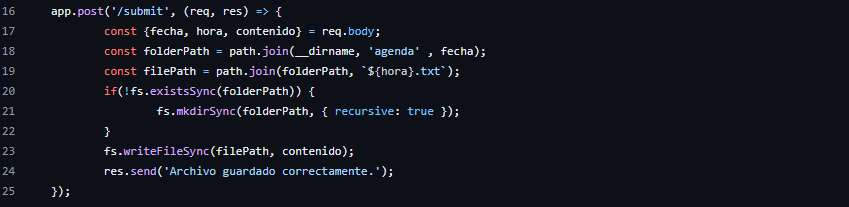
\includegraphics[width=\textwidth]{img/2.png}
\item \textbf{app.get('/buscar' ... ): } Esta petición es la primera parte de la sección Editar. Esta solo recibe 2 atributos(fecha, hora) y con estos verifica que el documento elegido exista, si es así se coloca el contenido del documento en el textarea continuo al botón para que el usuario pueda editar el documento ya presente, caso contrario se notifica que no existe un documento con los datos enviados.\\



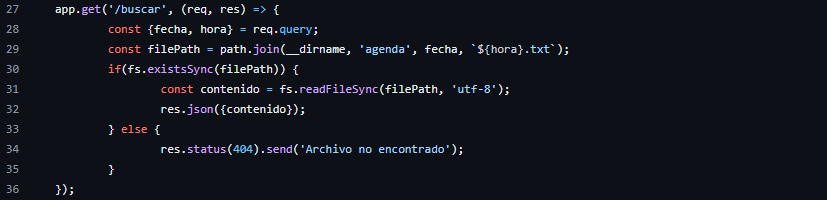
\includegraphics[width=\textwidth]{img/3.png}
\item \textbf{app.post('/editar' ...): } Esta petición es la segunda parte de la sección Editar. Tras la verificación de la petición anterior y con el texto ya modificado, al presionar el botón de enviar se mandaran los 3 atributos(fecha, hora, contenido) como en la petición /submit, y tras ubicar al archivo se reescribirá el mismo pero con el nuevo contenido entregado por el usuario.\\



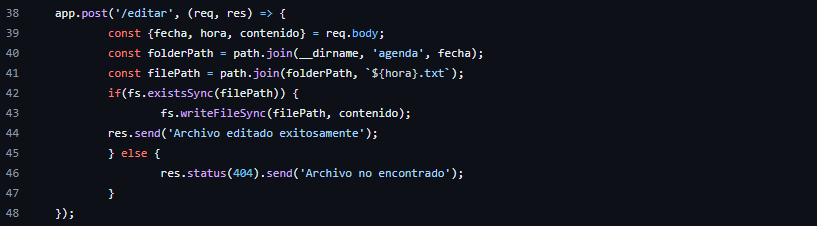
\includegraphics[width=\textwidth]{img/4.png}
\item \textbf{app.post('/eliminar' ... ): } Esta petición se encarga de eliminar los eventos. Para ello se reciben 2 atributos(fecha, hora), con los cuales se ubicará al documento para luego proceder a eliminarlo de su carpeta designada. \\



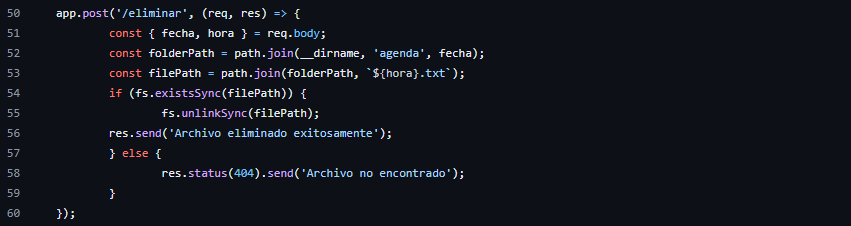
\includegraphics[width=\textwidth]{img/5.png}
\item \textbf{app.get('/arbol' ...): } Esta petición se encarga de realizar el proceso para retornar el árbol que contiene a los directorios y documentos. Este llama a la función crearArbol() mandando como atributo la dirección del directorio, la cual retorna un árbol de su contenido con el formato pedido en la práctica.\\



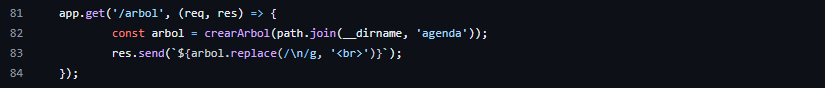
\includegraphics[width=\textwidth]{img/6.png}
\item \textbf{crearArbol(): } Esta función lee el contenido del directorio actual, creando una constante la cual contendrá el árbol a devolver. Se itera sobre cada elemento, donde dependiendo si es carpeta o documento se colocará un prefijo -guiones u otros, y se utilizan | para indicar la jerarquía de carpetas y documentos.\\



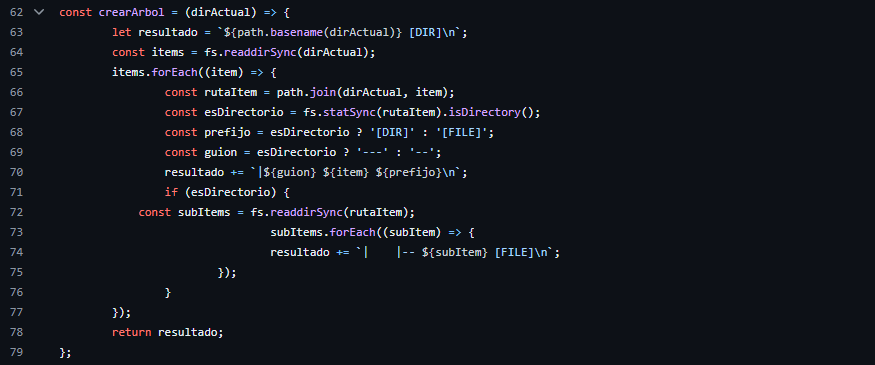
\includegraphics[width=\textwidth]{img/7.png}
\end{itemize}

\subsection*{Funcionamiento de la Página Web.}

\begin{itemize}
\item \textbf{Página Web:} \\



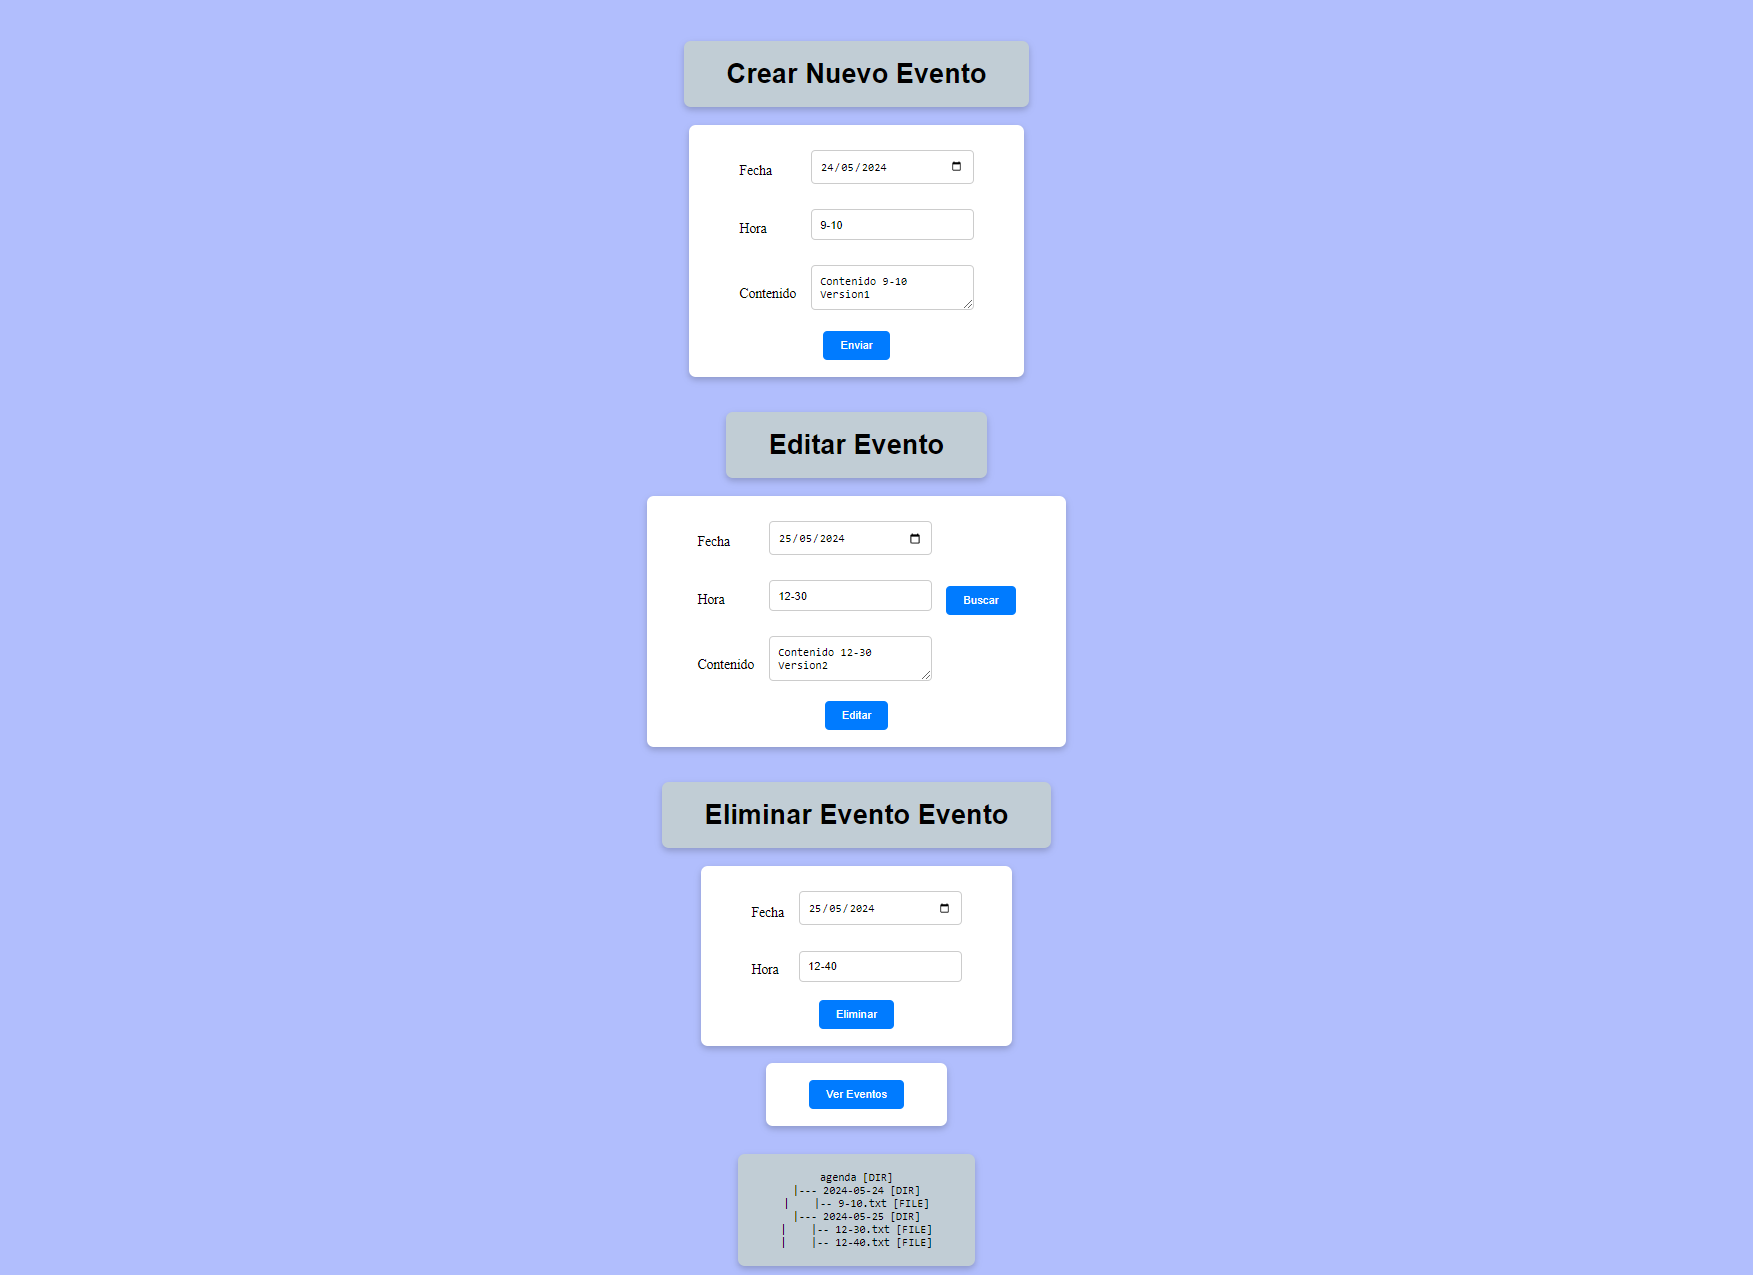
\includegraphics[width=\textwidth]{img/8.png}
\item \textbf{Probando Creación de Eventos:} \\




\includegraphics[width=\textwidth]{img/9.png}



\includegraphics[width=\textwidth]{img/10.png}
\item \textbf{Probando Edición de Eventos:} \\



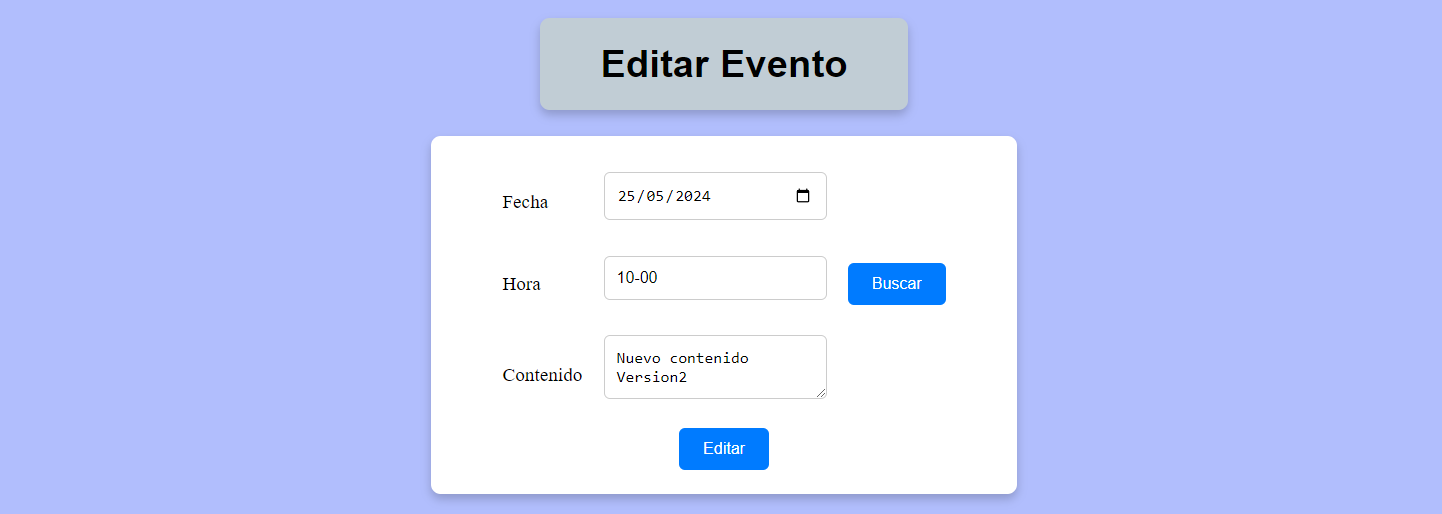
\includegraphics[width=\textwidth]{img/11.png}



\includegraphics[width=\textwidth]{img/12.png}
\item \textbf{Probando Eliminación de Eventos:} \\




\includegraphics[width=\textwidth]{img/13.png}



\includegraphics[width=\textwidth]{img/14.png}
\end{itemize}
\subsection*{Pregunta.}
Mencione la diferencia entre conexiones asíncronas usando el objeto XmlHttpRequest, JQuery.ajax y Fetch. Justifique su respuesta con un ejemplo muy básico. Eje: Hola Mundo, IMC, etc.
\begin{itemize}
\item \textbf{XmlHttpRequest: } Es la API original de JavaScript, requiere manejar de forma manual múltiples eventos.\\



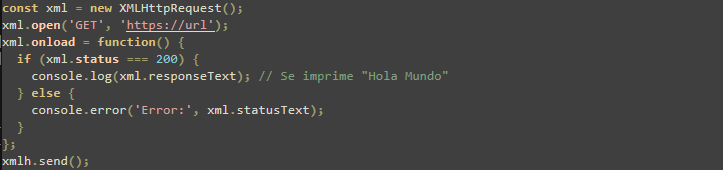
\includegraphics[width=\textwidth]{img/xml.png}
\item \textbf{JQuery.ajax: } Es una biblioteca de JavaScript, la cual usa la función \$.ajax al configurar objetos.\\




\includegraphics[width=\textwidth]{img/ajax.png}
\item \textbf{Fetch: } Es la API más moderna. Su funcionamiento viene acompañado de "promesas", manejando respuestas como .then y .catch.\\



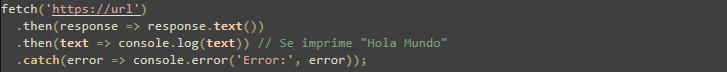
\includegraphics[width=\textwidth]{img/fetch.png}
\end{itemize}
\section{Commits realizados:}





\includegraphics[width=\textwidth]{img/commits.png}
\section{Rúbrica:}




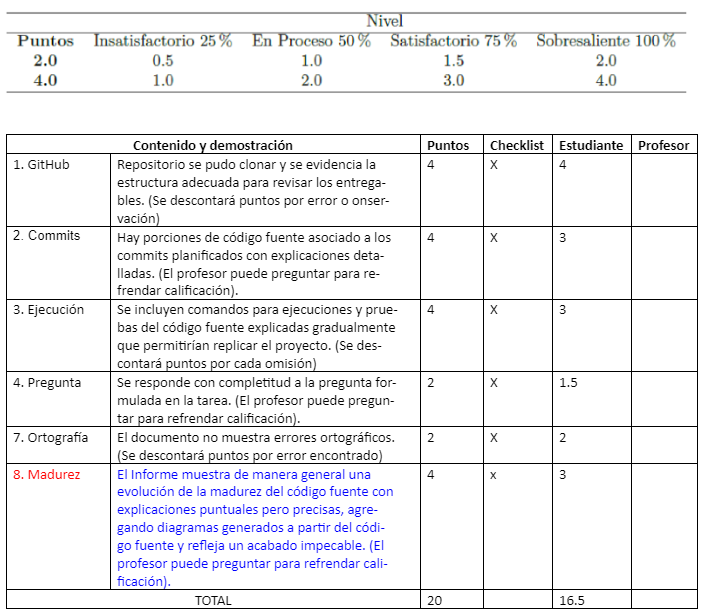
\includegraphics[width=\textwidth]{img/rubrica.png}
\end{document}